% ANLP M26 Assignment 1 - final report
\documentclass[12pt]{article}
%\usepackage{fontspec}
%\setmainfont{Times New Roman}
\usepackage[margin=1in]{geometry}
\usepackage{mathptmx}
\usepackage{graphicx,booktabs,amsmath,hyperref,enumitem}
\usepackage{xcolor,titlesec}
\titlespacing*{\section}{0pt}{9pt plus 2pt minus 2pt}{5pt}
\titlespacing*{\subsection}{0pt}{7pt plus 2pt minus 2pt}{4pt}
\hypersetup{colorlinks=true,linkcolor=blue,urlcolor=blue}


% ANLP M26 Assignment 1 - final report
\title{Assignment 1}
\author{Ojas Kataria\\2024114008}
\date{}

\begin{document}
\maketitle

\href{https://wandb.ai/irishbumfuzzle-team/anlp-assignment1/workspace?nw=nwuseririshbumfuzzle}{WandB},
\href{https://huggingface.co/irishbumfuzzle/anlp-a1-C1}{HF C1},
\href{https://huggingface.co/irishbumfuzzle/anlp-a1-C2}{HF C2},
\href{https://huggingface.co/irishbumfuzzle/anlp-a1-C3}{HF C3},
\href{https://huggingface.co/irishbumfuzzle/anlp-a1-C4}{HF C4},
\href{https://huggingface.co/irishbumfuzzle/anlp-a1-C5}{HF C5}

\section{Task and approach}
We are given 5000 lines of the Brown corpus and their
ciphertexts, produced by a repeating-key XOR cipher with the 8-byte key
\texttt{ANLP2026}: byte $i$ of the ciphertext is $C[i] = P[i] \oplus K[i \bmod 8]$,
provided as a bit string. Built a Transformer
with BPE tokenization on the ciphertext side, and run a
five-way ablation in which each configuration changes exactly one component of
the base model C1 (Table~\ref{tab:configs}).

\begin{table}[h]
\centering\small
\setlength{\tabcolsep}{4.5pt}
\caption{Ablation configurations (all else shared).}
\label{tab:configs}
\begin{tabular}{lllll}
\toprule
Config & Positional & Attention & Normalization & Tokenization \\
\midrule
C1 Base    & Sinusoidal & MHA ($h{=}8$) & LayerNorm & BPE 512 + byte target \\
C2 RoPE    & RoPE       & MHA ($h{=}8$) & LayerNorm & as C1 \\
C3 GQA     & Sinusoidal & GQA ($h{=}8$, kv$=4$) & LayerNorm & as C1 \\
C4 RMSNorm & Sinusoidal & MHA ($h{=}8$) & RMSNorm   & as C1 \\
C5 BLT     & Sinusoidal & MHA ($h{=}8$) & LayerNorm & token-free 4-byte patches \\
\bottomrule
\end{tabular}
\end{table}

All configurations share the config: $d_{model}{=}256$, 8 heads,
4+4 layers, FFN 1024, dropout 0.1, learning rate $5\cdot10^{-4}$ (250-step warmup,
cosine decay to $10^{-5}$), AdamW (weight decay $10^{-2}$), effective batch 16,
max source 1024 tokens; Evaluation is greedy decoding on the held-out test
set: bit-level accuracy, exact-sequence accuracy, mean Levenshtein distance,
character-level BLEU and ROUGE-L.

Three main points. \emph{First}, the BPE merge vocab is the most influential in metrics:
at an 8000 vocabulary all configs plateau at $\approx$0.69 greedy
bit accuracy (0.927 teacher-forced); shrinking vocab size to 512 lifts C1 to 0.9996
bit / 97.2\% exact sequence. \emph{Second}, at the 1:1
vocabulary RoPE is clearly worse than sinusoidal (0.9663), GQA slightly worse
(0.9969), and RMSNorm indistinguishable from LayerNorm (0.9981). \emph{Third}, the
token-free, non-autoregressive Byte Latent Transformer (BLT) config C5 reaches
0.9999 bit accuracy, while training $\approx$5$\times$
faster and using \emph{less} GPU memory per line than C1
(Section~\ref{sec:blt}), at a cost of 3.8 points of exact-sequence accuracy.

\section{Design decisions}
\label{sec:design}
\paragraph{Ciphertext: learned BPE over a phase-annotated byte alphabet.}
Applied byte-level BPE to the ciphertext bytes enriched with the key phase: the
symbol at byte index $i$ is $(b, i \bmod 8)$, a 2048-symbol alphabet of which 424
occur. Since the phase is a deterministic function of position, decryption
becomes a \emph{per-symbol} lookup, $b \oplus K[p]$; without the annotation the
model must additionally regress $i \bmod 8$ from context.

\paragraph{Vocabulary size: 512}
A 512 vocabulary holds all 424 base symbols plus 88 learned merges (0 UNK on
every split). An 8000-vocabulary token spans 2--5 bytes, so a wrong greedy prefix
corrupts both the content and the ordinal mapping from token index to byte index,
making mislocalisation permanent. The smaller input
embedding also cuts the autoregressive parameter count from 9.54M to 7.63M.

\paragraph{Target: one token per plaintext byte.}
A second BPE vocabulary on the plaintext side \emph{collapses to the English
prior}: 0.668 bit accuracy after 40 epochs (always-space baseline: 0.662) despite
falling teacher-forced loss, the model must first align two independent
segmentations of $\sim$200--1000 positions (boundary intersection-over-union 0.41)
before it can learn the cipher.

\paragraph{C5: fixed 4-byte patches.}
C5 uses BLT: raw ciphertext bytes (no subword tokenization) in
fixed 4-byte patches (final patch: 1--4 bytes). Decoding is
\emph{non-autoregressive}: all target positions in a single pass.

\section{Problem with 8k vocab size}
\label{sec:exposure}
Using 8000 BPE vocabulary. There C1 showed a
large teacher-forced/greedy gap: 0.927 vs 0.690 bit accuracy at 40 epochs, greedy
validation nearly flat (0.679 at epoch 10 to 0.691 at epoch 40) while teacher
forcing climbed steadily; greedy outputs start correctly and then degenerate
into fluent but unrelated English. randomizing
10\% of prefix positions costs 0.10; at 100\% random the model is \emph{below} the
always-space baseline (0.654 vs 0.662). The decoder uses the \emph{content} of
its own prefix to locate the source position: one wrong byte and it never
re-locates, falling back to the English prior.

\emph{Random prefix dropout} (replacing a fraction $q$
of decoder-input prefix ids with random ids): $q{=}0.5$ barely moves greedy
(0.679) and hurts teacher forcing (0.774); $q{=}1.0$ collapses to the prior
(0.662/0.657), random noise is not the distribution of greedy errors, which
are \emph{plausible} wrong bytes. \emph{Scheduled sampling} (feed each sample its
own cached greedy prefix with probability ramping $0\to0.5$ over 8 epochs) does
not help either: greedy 0.664, teacher forcing 0.814, any corrupted prefix
fraction makes the model distrust a correct prefix without teaching
re-localization.

The resolution is the tokenizer itself. At 512 vocabulary the same C1 has a
teacher-forced/greedy gap of only 0.016 at epoch 10 (0.9666 vs 0.9506) and
essentially zero by epoch 40 (both 1.0000 on validation); greedy accuracy climbs
0.9506 (ep 10) $\to$ 0.9937 (ep 20) $\to$ 1.0000 (ep 40). With multi-byte source
tokens a wrong prefix corrupts the content \emph{and} the token-index$\to$byte-index
mapping, so mislocalisation is permanent; with 1:1 tokens the decoder's own depth
still tells it where it is, so errors do not compound. The 8000-vocabulary runs
are retained as a tokenization ablation (Table~\ref{tab:main}, right).

\begin{table}[t]
\centering\footnotesize
\caption{C1 (8000-vocab source), epoch-25 checkpoint, 30-line validation sweep:
what the decoder is fed as its prefix. Bit accuracy.}
\label{tab:prefix}
\begin{tabular}{lr}
\toprule
Decoder prefix & Bit acc. \\
\midrule
oracle (ground truth)               & 0.893 \\
10\% of prefix positions randomised & 0.791 \\
50\% randomised                     & 0.688 \\
100\% randomised                    & 0.654 \\
resync to oracle every 2 bytes      & 0.767 \\
resync to oracle every 10 bytes     & 0.691 \\
pure greedy (own prefix)            & 0.676 \\
always-space baseline               & 0.662 \\
\bottomrule
\end{tabular}
\end{table}

\section{Setup}
\label{sec:setup}

\textbf{Model.} $d_{model}{=}256$, 8 heads (C3: 4 key/value heads), 4+4 layers,
FFN 1024, dropout 0.1. Parameter counts: C1/C2 7.63M, C4 7.62M, C3 7.10M, C5 5.55M.

\textbf{Training.} AdamW ($\beta_2{=}0.98$, weight decay $10^{-2}$), peak lr
$5\cdot10^{-4}$, 250-step warmup, cosine decay to $10^{-5}$, gradient clipping
1.0, effective batch 16, C1--C4 use microbatch 8 $\times$ 2 gradient-accumulation
steps, C5 uses microbatch 16, 40 epochs for C1--C4. C5 trained on 120-epochs;

\section{Results}
\label{sec:results}
\begin{table}[t]
\centering\footnotesize
\setlength{\tabcolsep}{4pt}
\caption{Test-set results, greedy decoding. Left: official 512-vocab study
(C1--C4: 468 lines; C5: 426 lines, 1024-byte raw-byte cap); right: identical
architecture at BPE 8000 (40 epochs; 500 lines; C5 has no 8000-vocab run).
Always-space baseline: bit acc 0.662.}
\label{tab:main}
\begin{tabular}{lrrrrrrr}
\toprule
 & \multicolumn{5}{c}{BPE 512 (official)} & \multicolumn{2}{c}{BPE 8000} \\
\cmidrule(lr){2-6}\cmidrule(lr){7-8}
Config & Bit & Seq & Lev. $\downarrow$ & BLEU & ROUGE-L & Bit & Seq \\
\midrule
C1 Base    & 0.9996 & \textbf{0.9722} & 0.12 & \textbf{0.9998} & \textbf{0.9999} & 0.6902 & 0.0060 \\
C2 RoPE    & 0.9663 & 0.7372 & 8.26 & 0.9909 & 0.9880 & 0.6773 & 0.0000 \\
C3 GQA     & 0.9969 & 0.8932 & 0.34 & 0.9991 & 0.9997 & 0.6905 & 0.0040 \\
C4 RMSNorm & 0.9981 & 0.9615 & 0.22 & 0.9997 & 0.9999 & 0.6902 & 0.0020 \\
C5 BLT     & \textbf{0.9999} & 0.9343 & \textbf{0.08} & 0.9996 & 0.9999 & -- & -- \\
\bottomrule
\end{tabular}
\end{table}

\begin{figure}[t]
\centering

\includegraphics[width=0.92\textwidth]{figures/training_curves.png}
\caption{T(a)~loss, (b)~bit accuracy, (c)~exact-sequence accuracy. C5 (purple)
converges fastest}
\label{fig:curves}
\end{figure}

Three readings of Table~\ref{tab:main}. \emph{First}, the tokenization axis
dominates: 8000$\to$512 lifts every autoregressive config by
$\approx$0.29--0.31 bit accuracy and sequence accuracy from 0--0.6\% to
73.7--97.2\% (Table~\ref{tab:main}, right), an order of magnitude larger than
any architectural effect. \emph{Second}, at the 1:1 vocabulary: RoPE (C2) is clearly
worst ($-$3.3 bit, $-$23.5 sequence points; best checkpoint epoch 39, validation
loss still 0.0022, not collapsed); GQA (C3) costs $-$0.27 bit / $-$7.9 sequence
points while halving the key/value heads; RMSNorm (C4) is within 1.1 sequence
points of LayerNorm. \emph{Third}, C5 is the strongest single result: best bit
accuracy (0.9999) and best Levenshtein (0.08 on 554-byte-median lines); C1 is
best on exact sequence (0.9722 vs 0.9343). C5's residual errors are scattered
single bytes ($\approx$0.006\% of positions), not drift; a 64-line overfit probe
drives its training loss to $5\cdot10^{-4}$ at 100\% bit accuracy, so capacity is
not the limit.

\begin{table}[t]
\centering\footnotesize
\caption{entropy-dynamic
(mean 4.0 bytes, $\theta_g{=}4.63$):}
\label{tab:c5patch}
\begin{tabular}{lrrrr}
\toprule
Patching & Bit acc. & Seq acc. & Lev. $\downarrow$ & Peak mem. \\
\midrule
fixed stride 4 & \textbf{0.9999} & \textbf{0.9343} & \textbf{0.08} & 4.27\,GB \\
entropy (dynamic)         & 0.9931 & 0.0305 & 14.0 & 4.54\,GB \\
\bottomrule
\end{tabular}
\end{table}

\subsection{C5 (BLT): the memory--accuracy tradeoff}
\label{sec:blt}
\begin{table}[t]
\centering\footnotesize
\setlength{\tabcolsep}{5pt}
\caption{}
\label{tab:cost}
\begin{tabular}{lrrrrr}
\toprule
Config & Peak mem. & Per line & Epoch & Throughput & Total \\
 & (GB) & (MB) & (s) & (lines/s) & (min) \\
\midrule
C1 Base    & 2.55 & 319 & 118 &  32 & 129  (40 ep) \\
C2 RoPE    & 2.54 & 318 & 124 &  31 & 141  (40 ep) \\
C3 GQA     & 2.53 & 316 & 117 &  32 & 122  (40 ep) \\
C4 RMSNorm & 2.51 & 314 & 115 &  33 & 118  (40 ep) \\
C5 BLT     & \textbf{4.27} & \textbf{267} & \textbf{24} & \textbf{147} & \textbf{46} (120 ep) \\
\bottomrule
\end{tabular}
\end{table}

\begin{figure}[t]
\centering
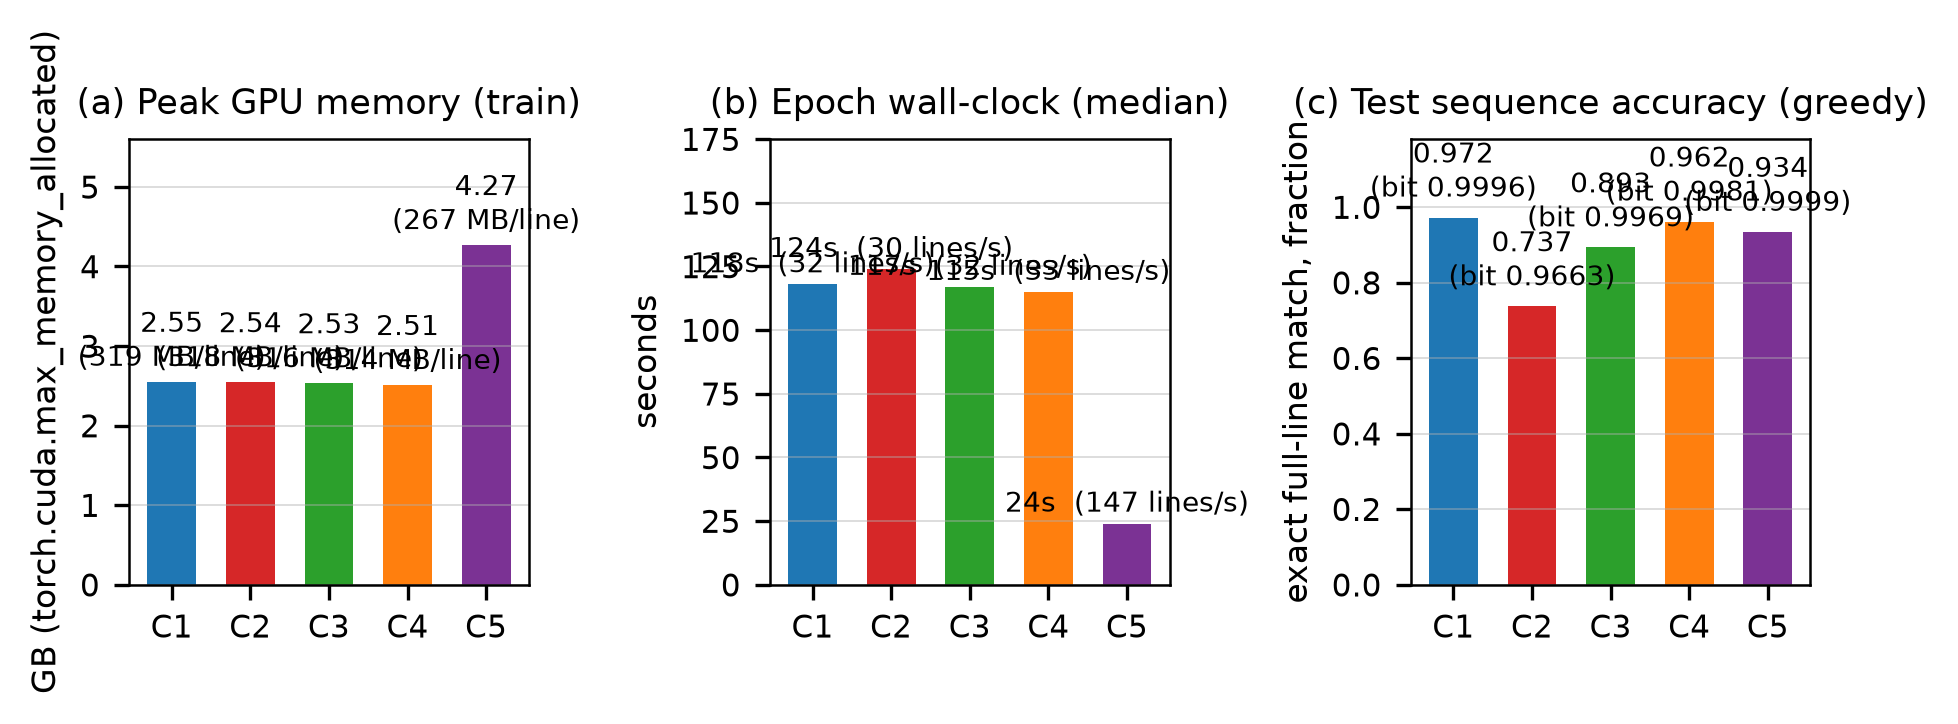
\includegraphics[width=0.95\textwidth]{figures/blt_tradeoff.png}
\caption{}
\label{fig:tradeoff}
\end{figure}

Comparing the C5 model against the baseline C1, focusing on training speed, peak GPU memory, and reconstruction quality. Overall, C5 delivers significant speed and structural efficiencies in exchange for a small drop in exact-match accuracy.

Memory
At first glance, C5's peak memory looks higher than C1's (4.27 GB vs. 2.55 GB). However, C5 is doing much more work at once: it processes double the microbatch size (16 lines vs. 8) and skips the activation checkpointing that C1 relies on (which saves C1 memory but costs it a ~30\% compute penalty).

When you look at the cost per line, C5 is actually lighter (267 MB vs. 319 MB). If we dropped C5 down to C1's batch size of 8, its peak memory would sit around 2.5 GB-matching C1, but without needing the checkpointing penalty. This efficiency is built into the architecture: C5 has 27\% fewer parameters (5.55M vs 7.63M) and processes patches in a single parallel pass, bypassing C1's heavier encoder-decoder setup.

Speed
C5 is roughly five times faster. A single epoch takes a median of 24 seconds (147 lines/s) compared to C1's 118 seconds (32 lines/s). To put that into perspective, a full 120-epoch run for C5 finishes in 46 minutes, while C1 needs 129 minutes just to finish 40 epochs.

This speed advantage comes from doing one parallel pass per line instead of autoregressive, step-by-step unrolling. The same advantage carries over to inference, where C1 requires up to 2,670 sequential steps while C5 only needs a single forward pass.

Accuracy
The trade-off for these speed and memory wins is a 3.8-point drop in exact-sequence accuracy (93.43\% for C5 vs. 97.22\% for C1). However, C5 actually beats C1 on both bit accuracy (99.99\% vs 99.96\%) and Levenshtein distance (0.08 vs 0.12).

This happens because C5's mistakes tend to be isolated, single-byte errors. These barely register in edit distance but automatically disqualify an exact sequence match. C1, by contrast, suffers from compounding prefix drift.

Ultimately, C5's token-free approach buys a 5$\times$ speed boost, lowers per-line memory, and requires fewer parameters, all for a minor exact-match tax. As an added bonus, its non-autoregressive design naturally eliminates exposure bias, since its test pass works exactly the same way as validation.

\section{Analysis}
\label{sec:discussion}
\paragraph{RoPE is the wrong inductive bias for this task.}
C2 is a genuine negative result: its teacher-forced accuracy is near-perfect by
epoch 30 (0.9993), yet its greedy trajectory stalls at $\approx$0.68 for 20
epochs, then jumps to 0.9249 (epoch 30) and 0.9592 (epoch 40), a
$\approx$4-point residual gap the sinusoidal configs never show. The residual
errors are late-line repetition loops (``\dots before transferring to No
Squadron before transferring to No Squadron\dots''). Decryption requires \emph{absolute}
target$\leftrightarrow$source alignment (output $i$ reads source $i$) over
hundreds of positions: sinusoidal codes give every position a stable identity in
both sequences, and the decoder still knows where it is when its own prefix is
wrong. RoPE encodes only \emph{relative} offsets; absolute position must be
integrated from a possibly wrong prefix, the step that fails at length. For
alignment-heavy long-sequence tasks, absolute encodings are the safer choice,
the reverse of the general-purpose LLM default, where the mapping is semantic.

\paragraph{GQA costs a little; RMSNorm is free.}
C3 halves the key/value heads (7.63M $\to$ 7.10M parameters) at a cost of 0.27
bit / 7.9 sequence points, consistent with a softer cross-attention position
index: 4 shared KV heads carry less position-locating information per head on a
task that \emph{is} position lookup. At larger scales GQA's inference-time win
usually dominates; at this budget MHA keeps more alignment precision. C4
(RMSNorm) is indistinguishable from LayerNorm within 1.1 sequence points and is
the sensible production default.

\paragraph{What the token-free baseline does and does not show.}
C5 works because the cipher is a deterministic per-byte function of
$(b, i \bmod 8)$: given the 1:1 alignment, each output is a local lookup with
context, and there is no autoregressive prefix to drift. Its single-pass test
decode is the same mode its validation used, so there is no train/decode
mismatch to diagnose, the exposure-bias axis is removed entirely.

\paragraph{The English-prior collapse, and where the budget runs out.}
Using BPE on both the input and output sides ultimately flatlines, barely edging out a naive "always-space" baseline (0.668 vs. 0.662). While the training loss looks like it is steadily improving, the small 4-layer model is actually just wasting its capacity trying to align two mismatched sets of token boundaries (boundary IoU 0.41) rather than learning the underlying cipher.

Dropping target tokenization entirely in favor of raw byte targets yielded the single biggest improvement in the study-jumping from 0.668 to 0.927 (and hitting 0.9996 with greedy decoding at a 512 vocabulary). The second biggest win came from using a phase-annotated source alphabet, which boosted accuracy from 0.62 to 0.90 in our 25-epoch test runs..

\end{document}

